\subsection{Key concepts of UVM-ML}

The primary goal of the UVM-ML open architecture solution is to expand the UVM scope from a single language to multiple
languages. Thereby it is independent of the simulator used and can be extended to support additional verification
languages. The main elements used in the multi-language library are the language frameworks, the framework adapters and
the multi-language backplane.
\begin{itemize}
  \item\textbf{Framework}\\
  Frameworks are the combination of the language and the methodology used to develop verification components. Some
  examples are UVM-SV, UVM-SystemC and UVM-\textit{e}.
  \item\textbf{Backplane}\\
  The backplane is the central component of the multi-language architecture and connects the frameworks in a star
  topology.
  It is only internal to UVM-ML and cannot be accessed directly by the user code.
  \item\textbf{Adapter}\\
  Adapters build the bridge between frameworks and the backplane. They provide all multi-language functionalities for
  the frameworks so they are unaware of the backplane.
\end{itemize}

\begin{figure}[htb]
 \centering
 %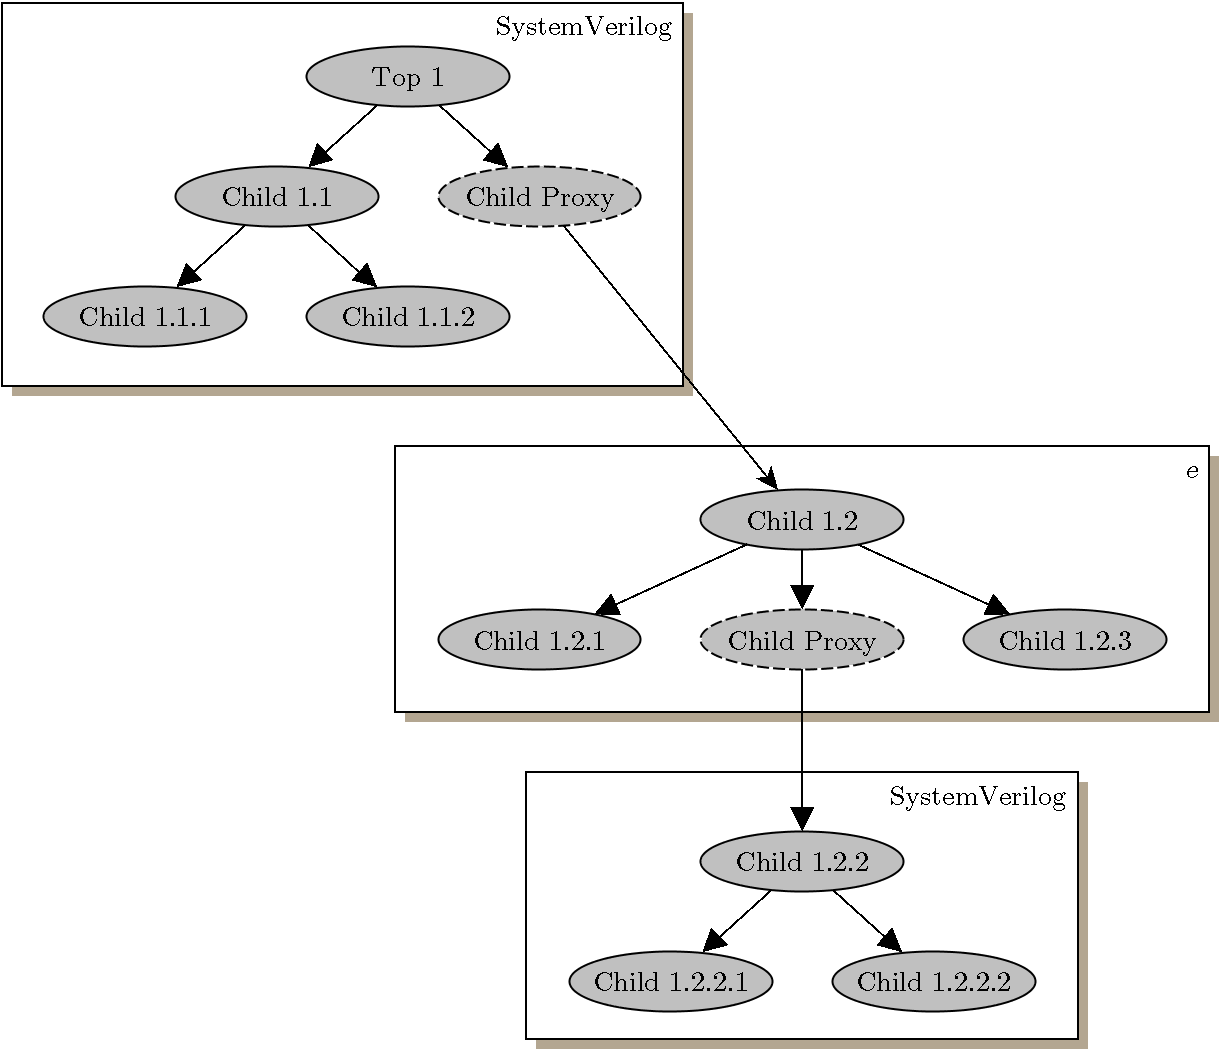
\includegraphics[width=1.0\textwidth,angle=0]{abb/UVM_ML_unified}
 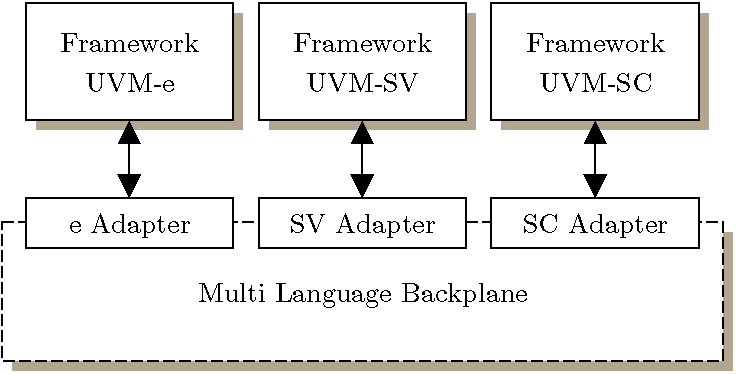
\includegraphics[scale=0.3]{abb/UVM_ML_architecture}
 \caption{UVM-ML architecture}
\label{fig:UVM_ML_architecture}
\end{figure}

The basic structure of the multi-language architecture is displayed in figure~\ref{fig:UVM_ML_architecture}. Each
framework accesses the backplane exclusively through its corresponding adapter. There are only the three adapters shown,
which are provided by the UVM-ML package, but it can be extended to support other frameworks as well.